\documentclass[fleqn]{article} 
\usepackage[a3paper,landscape,vmargin=1.0cm,hmargin=1.5cm]{geometry} 

\usepackage{latexsym}
\usepackage{graphicx}
\usepackage{latexsym}

\usepackage{multicol}

\usepackage{epsfig}
\usepackage[dvips,xdvi]{color}

\usepackage{amsmath}
\usepackage{amssymb}

%--------------------------------------------------------------
	\setlength{\textwidth}{1120pt}
	\setlength{\textheight}{790pt}
%--------------------------------------------------------------
	\setlength{\oddsidemargin}{-50pt}
	\setlength{\evensidemargin}{-50pt}
%--------------------------------------------------------------
	\setlength{\topmargin}{-70pt}
	\setlength{\headheight}{0pt}
	\setlength{\topskip}{0pt}
%--------------------------------------------------------------
	\setlength{\columnseprule}{0.5pt}
	\setlength{\columnsep}{10pt}
%--------------------------------------------------------------
	\renewcommand{\baselinestretch}{1}
%--------------------------------------------------------------
	\setlength{\mathindent}{0.5cm}
	\setlength{\parindent}{7pt}
%--------------------------------------------------------------
	\renewcommand{\bottomfraction}{0.99}
	\renewcommand{\topfraction}{0.99}
	\renewcommand{\textfraction}{0.01}
%--------------------------------------------------------------
	\pagestyle{empty}
%--------------------------------------------------------------


%----------------------------------------------------------------
%	definition
%----------------------------------------------------------------
%----------------------------------------------------------------
%   equation 環境
%----------------------------------------------------------------
%		\def\topmat{\ \\ \vspace{-4mm}}
%		\def\botmat{\ \\ \vspace{-2mm}}
%		\def\bes{\vspace*{2mm}}
%		\def\ees{\ \\[-2mm]}
	%........................................................
	% equationの環境設定(\be,\ee)
	%      例 \bea 式 & 式 & 式 \nonumber\\ 式 & 式 & 式 \eea
	%........................................................
%		\def\be{\\ \ \\[-12mm] \begin{equation}}
%		\def\ee{\end{equation} \ \\[-11mm]}
		\newcommand{\be}{\begin{equation}}
		\newcommand{\ee}{\end{equation}}
	%........................................................
	% eqnarrayの環境設定(\bea,\eea)
	%      例 \bea 式 & 式 & 式 \nonumber\\ 式 & 式 & 式 \eea
	%........................................................
%		\def\bea{\\ \ \\[-16mm] \begin{eqnarray}}
%		\def\eea{\end{eqnarray} \ \\[-13mm]}
		\newcommand{\bea}{\begin{eqnarray}}
		\newcommand{\eea}{\end{eqnarray}}
	%........................................................
	% 番号なしeqnの環境設定(\nbe,\nee)
	%      例 \nbe 式 \\ 式  \nee
	%........................................................
%		\def\nbe{\\ \ \\[-12mm] \[}
%		\def\nee{\] \ \\[-11mm]}
		\newcommand{\nbe}{\[}
		\newcommand{\nee}{\]}
	%........................................................
	% matrixの入力(\bmatrix,\ematrix)
	%	例 \bmatrix{cc} 1&2\\3&4 \ematrix
	%........................................................
		\renewcommand{\bmatrix}{\left[\begin{array}}
		\newcommand{\ematrix}{\end{array}\right]}
	%........................................................
	% Greek character
	%........................................................
		\def\gggm{\mu}
		\def\ggge{\varepsilon}
		\def\gggw{\omega}
		\def\gggh{\theta}
		\def\ggga{\alpha}
		\def\gggb{\beta}
		\def\gggc{\gamma}
		\def\gggd{\delta}
		\def\gggp{\phi}
	%........................................................
	% others
	%........................................................
%		\def\half{\frac{1}{2}}
		\def\defeq{\stackrel{\rm def}{=}}


\renewcommand{\baselinestretch}{0.8}



%================================================================
\begin{document}
%================================================================
\rightline{
線形システム制御理論（2023.06.02)
\hspace{3cm}
\underline{学籍番号：　　　　　　　　　　　}
\hspace{1cm}
\underline{氏名：　　　　　　　　　　　　　}
\hspace{2cm}
}
%================================================================
\begin{multicols}{4}
%================================================================
\begin{enumerate}
%================================================================


%================================================================
\item
次の状態方程式
%\vspace{-3mm}
\begin{align}
	\frac{dx}{dt} 
	& =	\bmatrix{rr}
			0 & 1  \\
			1 & -1 
		\ematrix
		x
		+
		\bmatrix{c}
			0 \\
			1
		\ematrix
		u 
\nonumber %\\[-8mm] \nonumber
\end{align}
に対して次の状態フィードバックを考える．
%\vspace{-3mm}
\begin{align}
	u & = \bmatrix{ccc} f_1 & f_2 \ematrix x
\nonumber %\\[-8mm] \nonumber
\end{align}

以下の問に答えよ．
\begin{enumerate}
\item
閉ループ系の状態方程式を示せ．
\vspace{6cm}

\item
閉ループ系の状態方程式の特性多項式を求めよ．
\vspace{6cm}

\item
閉ループ系の極が$-1$, $-2$となる状態フィードバックを求めよ．

\end{enumerate}
%================================================================
\vfill\null
\columnbreak
%================================================================







%================================================================
\item
次のシステムに対してオブザーバを設計したい．
\begin{align}
	\frac{dx}{dt}
	&=	\bmatrix{cc}
			0 & 1 \\
			1 & 2
		\ematrix
		x
		+
		\bmatrix{c}
			1 \\
			1 
		\ematrix
		u
\nonumber \\
	y 
	&=	\bmatrix{cc}
			0 & 1 
		\ematrix
		x
\nonumber 
\end{align}

\begin{enumerate}

\item 
オブザーバゲイン$K$の次元に注意してオブザーバの状態方程式を示せ．
\vspace{5cm}

\item
オブザーバの極（推定誤差の収束速さ）が$-1$, $-2$となるようにオブザーバゲイン$K$を求めよ．
\vspace{8cm}

\end{enumerate}
%================================================================
\vfill\null
\columnbreak
%================================================================




%================================================================
\item
次の１次元システム
%\vspace{-1mm}
\begin{align}
	\frac{dx}{dt} &= 2 \cdot x + 1 \cdot u
	\ \ \ \  (A=2, B=1) 
\nonumber
%\vspace{-4mm}
\end{align}
に対して評価関数
%\vspace{-1mm}
\begin{align}
	J &= \int_0^\infty x^2 + r \cdot u^2 dt
	\ \ \ \  (Q=1, R=r)
\nonumber
%\vspace{-4mm}
\end{align}
を最小化する最適フィードバック
%\vspace{-1mm}
\begin{align}
	u=Fx
\nonumber
%\vspace{-4mm}
\end{align}
を求め，その性質について調べたい．
%\vspace{-2mm}

\begin{enumerate}
\item 
最適制御を求めるためのRiccati方程式を示せ．
\vspace{3cm}

\item
Riccati方程式の正定解$P>0$を求めよ．
\vspace{8cm}

\item
最適フィードバック$u=Fx$を求めよ．
\vspace{4cm}

\item
最適フィードバック$u=Fx$を施した後の閉ループ系の状態方程式を求めよ．
\vspace{4cm}

%================================================================
\vfill\null
\columnbreak
%================================================================

\item
閉ループ系の極を求めよ．
\vspace{2cm}

\item
$r\rightarrow 0$としたときの閉ループ系の極を求めよ．
\vspace{2cm}

\item
$r \rightarrow \infty$としたときの閉ループ系の極を求めよ．
\vspace{2cm}

\item
$r\rightarrow 0$, $r \rightarrow \infty$なる評価関数を用いるということはどのような制御系を設計することに対応するのか，それぞれについて簡潔に述べよ．
\vspace{1cm}
\end{enumerate}
%================================================================


　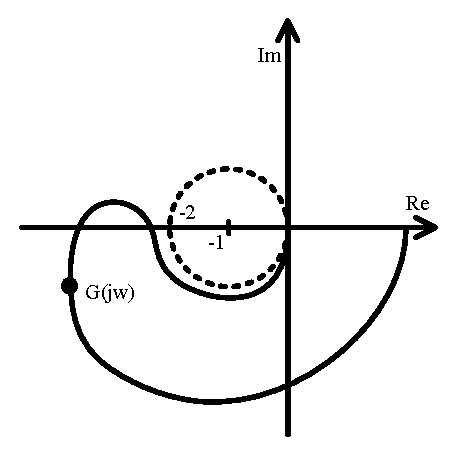
\epsfig{file=nyquist_prob.eps,scale=0.6}


\vspace{-2cm}
%================================================================
\item
Riccati方程式を変形することにより最適制御の一巡伝達関数$G(s)$が$|1+ G(j\omega)|>1$を満たすことが証明できる．これを用いて以下の問いに答えよ．
\begin{enumerate}
\item
この条件を満たす$G(j\omega)$のベクトル軌跡は下図のようになる．$1+G(j \omega)$のベクトルを図に記入し，このベクトル軌跡を説明せよ．（下図は元のシステムが安定である場合を示している）
\vspace{5cm}
\item
最適制御のゲイン余裕は$1/2$から$\infty$である（入力のゲインが$1/2$〜$\infty$まで変化しても閉ループ系の安定性が保たれる）ことを説明せよ．
\end{enumerate}
%================================================================




%================================================================
\end{enumerate}
%================================================================
\end{multicols}
%================================================================
\end{document}
%================================================================

